\chapter{Indirekte Fernlokalisierung mit 802.11}
\label{ch:phase1}
In einem ersten Schritt sollten laut Aufgabenstellung keine Veränderungen an den Access Points vorgenommen werden können.
Weil die Ortung deshalb auf WLAN basieren muss sind die Basisstationen im Folgenden immer APs. 
%TODO Ein Tag ist eine mobile Einheit, umgekehrt gilt dies jedoch nicht, da auch alle anderen WLAN-fähigen Geräte, wie Smartphones und Laptops, eine mobile Einheit sein können. \\
Die Unveränderlichkeit bedeutet insbesondere auch, dass keine Messwerte verwendet werden können, die direkt am AP gemessen werden und nicht als Teil der 802.11 Spezifikation in das dahinterliegende Netzwerk weitergeleitet werden.
Da time of arrival Synchronisation und präzise Timer bei den APs vorraussetzt und time difference of arrival nur von den APs gemessen werden kann, eignen sich diese Messgrößen nicht für diese Aufgabenstellung.
Received signal strength und roundtrip time of flight können auf der mobilen Einheit gemessen werden, nicht jedoch an den APs, da die in der PHY- beziehungsweise MAC-Schicht gemessenen Werte nicht an weitere Empfänger im Netzwerk propagiert werden. 
Somit scheidet die direkte Fernlokalisierung mangels Messgrößen aus, es wird stattdessen eine indirekte Fernlokalisierung durchgeführt bei der die mobile Einheit eine Selbstlokalisierung durchführt und das Ergebnis dem Ortungsserver über eine Datenverbindung mitteilt.

\begin{figure}[h]
  \centering
	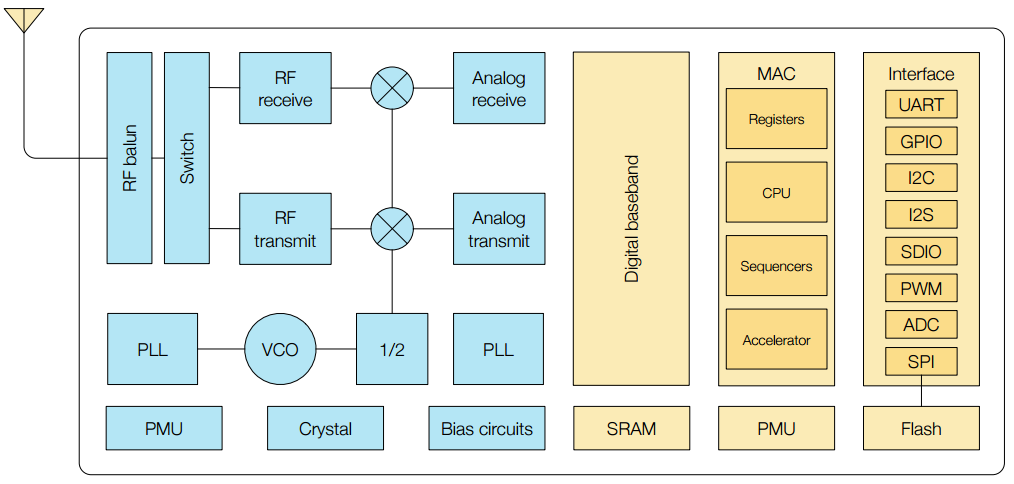
\includegraphics[width=\textwidth]{images/espblock.png}
  \caption{Blockdiagramm des ESP8266, aus \cite{espressif2017esp8266}}
  \label{fig:espblock}
\end{figure}

\section{ESP8266}
Der ESP8266 soll als Hardware für das Tag eingesetzt werden, dabei handelt es sich um einen Microcontroller von Espressif.
Der ESP8266 besitzt neben einer CPU eine 802.11b/g/n"-/e/i-fähige WLAN-Einheit und beherrscht diverse andere, kabelgebundene Kommunikationsstandards wie zum Beispiel GPIO, I2C und SPI, siehe Abb. \ref{fig:espblock}. \\
Da der ESP8266 selbst weder über Flashspeicher, noch über eine Antenne verfügt wird er auf einem Modul mit diesen Komponenten verbaut. 
Die in dieser Arbeit betrachteten Module sind das ESP12-S und das ESP12-F.
Das neuere ESP12-F sollte eine höhere Reichweite bei der Funkübertragung entfalten, dies wird noch Gegenstand eines Experiments sein.
%TODO Antennen markieren
Abb. \ref{fig:espmodules} zeigt die beiden Module nebeneinander, die unterschiedlichen Antennenformen sind deutlich zu erkennen.\\
Espressif gibt im Datenblatt auch Aufschluss über den Energieverbrauch des ESPs, siehe dazu Abb. \ref{fig:esppower}.
Für die Prototypenentwicklung wird ein ESP12-S Modul auf einem Adafruit Feather Huzzah verwendet, dieses stellt mit dem CP2104 eine serielle Verbindung zum ESP her, reguliert die Spannung für das Modul auf 3,3V und bringt den 2mm Pinabstand des ESP12-S Moduls auf die für Breadboards üblichen 2,5mm.
Das Adafruit Feather Huzzah mit ESP12-S ist in Abb. \ref{fig:espmodules} links abgebildet.

\begin{figure}[h]
  \centering
	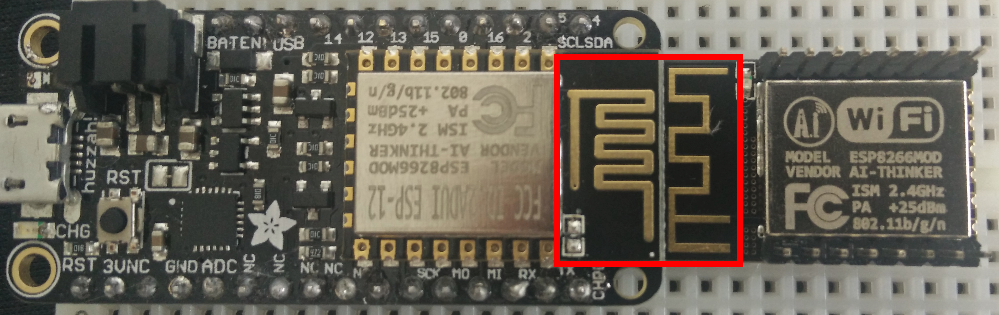
\includegraphics[width=\textwidth]{images/espmodules.png}
  \caption{Vergleich der Antennen, links: ESP12-S verbaut auf einem Adafruit Feather Huzzah, rechts: ESP12-F}
  \label{fig:espmodules}
\end{figure}

\begin{figure}[h]
  \centering
	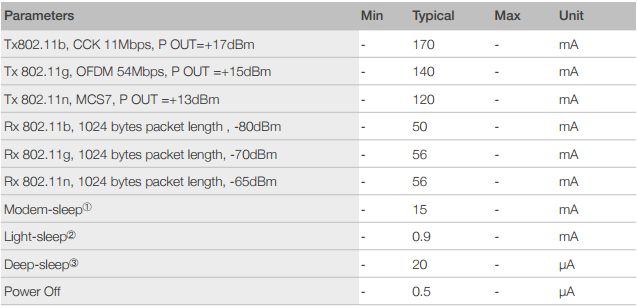
\includegraphics[width=\textwidth]{images/esppower.png}
  \caption{Energieverbrauch des ESP8266 bei verschiedenen Operationen, aus \cite{espressif2017esp8266}}
  \label{fig:esppower}
\end{figure}


\subsection{ESP8266 Arduino Core}
Eine einfache Möglichkeit den ESP8266 zu programmieren stellt die bekannte Arduino IDE dar \cite{banzi2017arduino}.\\
Unter Windows muss zunächst der Treiber für den \textit{CP2104 USB-to-Serial Chip} installiert werden, auf Linux und Mac entfällt dieser Schritt \cite{fried2017feather}.
Nach der Installation der Arduino IDE muss dort in den Einstellungen unter \textit{Additional Boards Manager URLs} die URL \url{http://arduino.esp8266.com/stable/package_esp8266com_index.json} hinzugefügt werden.  
Nach einem Neustart der IDE kann im \textit{Boards Manager} das Paket für den ESP8266 heruntergeladen werden und anschließend das Board \textit{Adafruit HUZZAH ESP8266} ausgewählt werden. \\
Ist das Board über USB mit dem Computer verbunden, kann nun eigener Code oder eines der Beispiele aus \textit{Examples for Adafruit HUZZAH ESP8266} mit STRG+U auf den ESP geladen werden. 
Dieser Vorgang wird im Folgenden als flashen bezeichnet. \\
Der ESP8266 Arduino Core wird als Open Source Projekt gepflegt und setzt die ESP Open SDK auf einen, für die Arduino IDE üblichen Stil um \cite{arduino2017core}. 
Dabei wird möglichst die Kompatibilität zu Arduino gewahrt, das führt oft dazu, dass bereitgestellte Funktionen der SDK nicht in Arduino umgesetzt wurden.
Sollten die Funktionen dennoch benötigt werden, können die Header-Dateien der SDK direkt importiert werden:

\begin{verbatim}
//Hier wird ein Header des ESP8266 Arduino Core importiert
#include <ESP8266WiFi.h> 

//Hier wird ein Header der ESP Open SDK importiert
extern "C" {#include "user_interface.h"} 
\end{verbatim}

Der ESP8266 Arduino Core wurde in der Version 2.3.0 verwendet.

\subsection{ESP Open SDK}
Statt mit der Arduino Core Umsetzung der ESP Open SDK kann natürlich auch direkt mit ihr programmiert werden \cite{esp2017open}. \\
Dazu muss zunächst das Github Projekt geklont werden: \texttt{git clone --recursive \url{https://github.com/pfalcon/esp-open-sdk}.git} und anschließend mit \texttt{make} kompiliert werden.
Wurde die Kompilierung erfolgreich abgeschlossen, sollte die Pfadvariable (PATH) entsprechend der Meldung des make-Tools erweitert werden. \\
Die in C geschriebenen Programme können nun mit einem modifizierten GCC-Kompiler kompiliert und anschließend mit dem esptool.py zunächst in ein Image umgewandelt und dann geflasht werden. 
Das in \textit{examples} enthaltene \textit{blinky} Beispiel beinhaltet neben dem Beispielcode eine Makefile, in der diese Schritte nachvollzogen werden können, mit \texttt{make flash} wird das Beispiel kompiliert und geflasht. \\
Programme werden in regulärem C unter Zuhilfenahme der in \texttt{/sdk/include} enthaltenen Header-Dateien geschrieben, zu beachten ist nur, dass einige Funktionen der \texttt{stdlib.h} nicht verwendet werden können.
Dies betrifft vor allem direkten Speicherzugriff wie zum Beispiel \texttt{memcpy}, hier muss stattdessen \texttt{os\_memcpy} verwendet werden.
Alle betroffenen Funktionen sind in \texttt{osapi.h} beschrieben. \\
Einige frühe Experimente zeigten, dass Programme, die mit der ESP Open SDK geschrieben wurden auf dem ESP schneller starten, als solche, die mit dem ESP8266 Arduino Core geschrieben wurden.
Diese Andeutung von Ineffizienzen bei der Übersetzung von Arduino Code wurde zum Anlass genommen, für die nachfolgenden Implementierungen nach der Fertigstellung des Prototypen in Arduino ebenfalls eine Implementierung in C hinzuzufügen, um ein optimales Programm zu erhalten. \\
Die ESP Open SDK wurde in der Version 2.0.0 verwendet.



\section{WiFi-LSS Implementierung}
Die mobile Einheit des WiFi-LLS Systems führt alle 5 Sekunden einen Scan aus, kodiert die Ergebnisse in XML und versendet sie an den Ortungsserver \cite{chen2007design}.
Da der Fokus dieser Arbeit auf dem Energieverbrauch liegt, werden für die Referenzimplementierung eines WiFi-LLS-Tags die Kodierung in XML durch eine simple String Kodierung ersetzt und die Ergebnisse werden über UDP an den Ortungsserver übermittelt. 
Damit wird der Overhead einer TCP-Verbindung vermieden.\\
Zunächst muss das Tag dem Netzwerk beitreten (Join), einen Scan ausführen und ein UDP-Paket versenden.
Da die Scan-Funktion des ESP8266 Arduino Core es nicht erlaubt den RSSI zu einem AP auszulesen muss \texttt{user\_interface.h} importiert und die Scan-Funktion der SDK direkt verwendet werden.
Um den Energieverbrauch weiter zu reduzieren, soll der ESP möglichst viel Zeit in Energiesparzuständen verbringen.
Der tiefste Schlafzustand, der dennoch eine Aufrechterhaltung der WLAN-Verbindung erlaubt ist der \texttt{light\_sleep}. 
Er wird vom ESP automatisch aufgerufen, wenn er keine Aufgaben zu erledigen hat.
Er kann aber auch manuell aufgerufen werden, beides wurde getestet.\\
Einige Parameter können gewählt werden. 
Die Intervallzeit bestimmt, wie oft der ESP aktiv ist und damit auch wie viel Energie er verbraucht.
Für Mitarbeiter im Tunnel kann von einer Maximalgeschwindigkeit von $30\ $km/h ausgegangen werden, diese wird durch Schienen- oder Lastkraftfahrzeuge erreicht. 
Die maximale Reichweite des ESP12-S beziehungsweise ESP12-F Moduls ist nicht bekannt und muss noch bestimmt werden, sie wird zwischen 50 und 100 Metern angenommen.
Es wurde daher ein Intervall von 5 Sekunden gewählt, in dieser Zeit bewegt sich ein Mitarbeiter bei 30 km/h ca. 42 Meter.\\
Des Weiteren kann theoretisch die Zahl der gescannten Kanäle gewählt werden. 
Da sich die Einflussbereiche der APs in einem WLAN-Netzwerk üblicherweise überlappen, ist es aber sinnvoll diese über die vier nichtüberlappenden Kanäle zu verteilen. 
Eine Implementierung, die nur einen Kanal scannt tritt deshalb nur außer Konkurenz an.\\
Tabelle \ref{table:llsconsumption} zeigt den gemessenen Energieverbrauch der Implementierungen in Arduino und C, jeweils mit und ohne manuell aufgerufenen \texttt{light\_sleep} und eine Implementierung, die nur einen Channel scannt.
Für die Tests wurde das Adafruit Feather Huzzah verwendet, es wurde mit 5 Volt aus einer USB-Powerbank mit Energie versorgt, der Verbrauch wurde mit einem dazwischen geschalteten TM103 USB-Power-Meter der Marke Muker gemessen. 
Jeder Versuch wurde mindestens eine Stunde durchgeführt.
Wurde in dieser Zeit der Verbrauchswert von 10 mAh nicht überschritten, wurde der Versuch verlängert, da der TM103 den Verbrauch ohne Nachkommastellen anzeigt.\\
Die Werte wurden stationär in einer Mietwohnung in einem fünfstöckigen Wohnhaus und damit nicht unter realen Bedingungen aufgezeichnet.
Unter realen Bedingungen finden durch die Bewegung des Mitarbeiters regelmäßig Reassizationen statt, im Gegenzug liefert ein Scan in einem Tunnel weniger Ergebnisse als in einem Wohnhaus.
Ein Test unter realen Bedingungen ist im Abschnitt \ref{kommtnoch} zu finden, er beinhaltet jedoch nur noch die Implementierung in C mit manuellem \texttt{light\_sleep} und einem Scan auf allen vier Kanälen.

%TODO Abstand Tabellenüberschrift
\begin{table}[h]
	\centering
	\caption{Energieverbrauch WiFi-LLS-artiger Tags}
	\label{table:llsconsumption}
	\begin{tabular}{p{3cm}|p{2.2cm}|p{1.5cm}|p{2cm}|p{2cm}|p{2cm}}
		SDK & manueller \texttt{light\_sleep} & Anzahl Kanäle & Spannung in V & $\varnothing$ Verbrauch in mA & $\varnothing$ Verbrauch in mW \\
		\hline
		Arduino Core & Nein & 4 & 5 & 22 & 110 \\
		Arduino Core & Ja & 4 & 5 & 21 & 105 \\
		ESP Open SDK & Nein & 4 & 5 & 19 & 95 \\
		ESP Open SDK & Ja & 4 & 5 & 19 & 95 \\
		\hline
		ESP Open SDK & Ja & 1 & 5 & 6,5 & 32,5 \\
	\end{tabular}
\end{table}

Die Tests zeigen, dass die Programmierung mit der ESP Open SDK einen Vorteil beim Energieverbrauch hat, dieser liegt bei ca 10\%.
Andererseits fällt auf, dass die Reduzierung der gescannten Channel eine signifikante Senkung des Energieverbrauchs nach sich zieht, die Scan-Funktion ist also der Hauptverbraucher.\\
Um die finale Laufzeit zu bestimmen muss die Kapazität des Akkus bekannt sein.

%TODO So ein Einfügungsblock.
Ein Lithium-Polymer Akku hat eine Nennspannung von 3,7 Volt, seine Kapazität wird in mAh angegeben, der Stromverbrauch wurde aber bei einer Spannung von 5 Volt gemessen. 
Das Feather Huzzah verwendet jedoch einen linearen Spannungsregler.
Für diesen gilt ein Wirkungsgrad $\eta \approx \frac{U_{ein}}{U{aus}}$ mit der ein- beziehungsweise ausgehenden Spannung $U_{ein/aus}$, da die eingehende Stromstärke $I_{ein}$ immer geringfügig über der ausgehenden Stomstärke $I_{aus}$ liegt \cite{streichert2012elektrik}.


Eine Milliamperstunde bei einer Eingangsspannung von 5 Volt kann also mit einer Milliamperstunde bei einer Eingangspannung bei 3,7 Volt gleichgesetzt werden.
Die Laufzeit für einen beispielhaften 1400 mAh Lithium-Polymer Akku beträgt also 1400\ mAh/19\ mA $\approx$ 73,68\ h.
Dies entpricht circa drei Tagen.


\section{Anpassungen für Bereichsortung}
\label{ch:phase1:sec:anpassungbereich}
Bei WiFi-LLS wird der Scan durchgeführt, um den RSSI zu nahen Access Points zu erhalten und dann auf dem Ortungsserver die Position der mobilen Einheit mit einer Trilateration zu berechnen.
Im Tunnel sind oft nur ein bis zwei APs in Reichweite, außerdem wird eine Bereichsortung als ausreichend angesehen. \\
Werden die APs geschickt den Bereichen zugeordnet, reicht das Wissen um einen nahen AP, um das Tag einem Bereich zuzuordnen.
Da dem Tag, die IP-Adresse seines Netztzugangs (Gateway) bekannt sein muss, kann dies als Ortungsinformation verwendet werden.
Die IP-Adresse wird nun zusammen mit der eigenen MAC-Adresse als Identifikator als String kodiert und per UDP an den Ortungsserver versendet.\\
Tabelle \ref{table:naiveconsumption} zeigt den gemessen Verbrauch der Implementierungen in Arduino und C, jeweils mit und ohne manuell aufgerufenen \texttt{light\_sleep}.

\begin{table}[h]
	\centering
	\caption{Energieverbrauch der Bereichsortungstags}
	\label{table:naiveconsumption}
	\begin{tabular}{p{3cm}|p{2.2cm}|p{1.7cm}|p{2.5cm}|p{2.5cm}}
		SDK & manueller \texttt{light\_sleep} & Spannung in V & $\varnothing$ Verbrauch in mA & $\varnothing$ Verbrauch in mW \\
		\hline
		Arduino Core & Nein & 5 & 14 & 70 \\
		Arduino Core & Ja & 5 & 7 & 35 \\
		ESP Open SDK & Nein & 5 & 6 & 30 \\
		ESP Open SDK & Ja & 5 & 5,5 & 27,5 \\
	\end{tabular}
\end{table}

Der Verbrauch liegt wie erwartet unter dem der WiFi-LLS Implementierung, sogar unter der Implementierung, die nur einen Kanal scannt.
Wird der selbe 1400 mAh beziehungsweise 1400 mAh Lithium-Polymer Akku angenommen, liegt die Laufzeit diesmal  bei 1400 mAh/5,5 mA $\approx$ 254,54 h, also bei über zehn Tagen. \\
Als weitere Optimierung könnte ein Tag nur dann senden, wenn eine Reassoziation stattgefunden hat.
Die mangelnde Transportsicherheit von UDP macht dieses Vorgehen jedoch riskant, wenn das Paket verloren geht wird kein Bereichswechsel erkannt.
Um wieder eine begrenzte Transportsicherheit zu erhalten, kann entweder das UDP-Paket mehrfach versendet werden; ohne Reassoziation in einen festen, aber größeren Intervall gesendet werden oder statt eine UDP-Verbindung eine TCP-Verbindung verwendet werden.
Somit ergeben sich neue Testszenarien: Ohne zusätzliche Sicherung, UDP-Paket mehrfach (dreifach) versenden, zusätzliches (30 beziehungsweise 60 Sekunden) Sendeintervall, TCP-Verbindung (offen halten oder nach dem Senden schließen). \\
Da der Verbrauch nun stark von der Anzahl der Reassoziationen abhängt sind im gegebenen, stationären Testszenario keine aussagekräftigen Ergebnisse möglich.
Dennoch sollen die Tests einen Ausgangswert ermitteln, dieser kann als untere Grenze für den Verbrauch einer Implementierung angesehen werden.
Da in den vorherigen Tests die Implementierungen mit der ESP Open SDK verbrauchsärmer waren, wurden alle in Tabelle \ref{table:naiveoptconsumption} gezeigten Implementierungen mit ihr erstellt, der manuelle \texttt{light\_sleep} ist immer aktiv.

\begin{table}[h]
	\centering
	\caption{Energieverbrauch der verbesserten Bereichsortungstags}
	\label{table:naiveoptconsumption}
	\begin{tabular}{p{3.5cm}|p{1.7cm}|p{2.5cm}|p{2.5cm}}
		Transportsicherung & Spannung in V & $\varnothing$ Verbrauch in mA & $\varnothing$ Verbrauch in mW \\
		\hline
		Ohne & 5 & 2 & 10 \\
		Dreifach UDP & 5 & 1,4 & 7 \\
		Zusatzintervall 30s & 5 & 2,62 & 13,1 \\
		Zusatzintervall 60s & 5 & 1,6 & 8 \\
		TCP (halten) & 5 & 1,2 & 6 \\
		TCP (schließen) & 5 & 1,07 & 5,35 \\
	\end{tabular}
\end{table}

Der Energieverbrauch sinkt durch das Einsparen von Sendevorgänge deutlich.
Für das Tag, das eine TCP-Verbindung öffnet, dem Ortungsserver seine Assoziation mitteilt und die Verbindung dann wieder schließt, ergibt sich für den angenommenen 1400\ mAh Lithium-Polymer Akku eine Laufzeit von 1400\ mAh/1,07\ mA $\approx$ 1308,41\ h. 
Dies entspricht gut 54 Tagen mit einer Akkuladung, diese werden jedoch in einem Szenario ohne Reassoziation erreicht.
Die tatsächliche Laufzeit muss unter realen Umständen gemessen werden, siehe dazu Abschnitt \ref{kommtnoch}.
Da die zusätzlichen Reassoziationen jedoch auch die vorherigen Implementierungen betreffen kann man schließen, dass Tags für die Bereichsortung durch die Ausnutzung von Assoziation und Reassoziation einen erheblich reduzierten Energieverbrauch gegenüber herkömmlichen Tags für die Trilateration aufweisen.




